\documentclass[12pt, letterpaper]{article}
\usepackage[a4paper, margin=1in]{geometry}
\usepackage{amsmath}
\usepackage{graphicx}
\usepackage{float}
\usepackage{hyperref}
\usepackage{caption}
\captionsetup[figure]{hypcap=true}
\graphicspath{{images/}}
\author{Joseph Yu}
\title{Reproducing CEBRA Results And Neural Alignment Analysis of CEBRA latents}
\begin{document}
\maketitle
\section{Introduction}
\label{sec:introduction}
At a high level CEBRA \cite{schneider2023} is a dimensionality reduction tool that leverages contrastive learning. CEBRA \cite{schneider2023} embeds neural responses into a latent space and then compares the latent embedding of the neural response with a positive sample and a negative sample. Using a combination of encoding and contrastive learning it is able to maximize the cosine distance between latent variables that correspond to different classes in the latent space. This proved to be especially effective in the context of reconstructing a video using frame ID classification from mouse V1 neural responses. The goal of this project is focused on the video reconstruction results of CEBRA \cite{schneider2023}. We broke down the project into three main parts. 
\begin{itemize}
    \item Understanding the dataset and doing some basic decoding of frame ID using simple classifiers.
    \item Training a VAE model to reconstruct the neural latents and then using the learned latents to reconstruct the video.
    \item Reproducing the results of CEBRA \cite{schneider2023} and then training a decoder to decode from CEBRA \cite{schneider2023} latents to the neural responses.
\end{itemize}

Through these steps our main goal of exploration is to first see how significant the CEBRA \cite{schneider2023} results are for decoding frame ID. At a first glance it seems like a simple classification problem. After answering the significance of CEBRA \cite{schneider2023} frame ID decoding performance we also want to explore if the learned neural latents are aligned with the true responses. This is important because CEBRA \cite{schneider2023} does not actually have a loss term that enforces the latents to be aligned with the true responses. If the latents are not aligned with the true responses then it is possible that the encoder is strictly learning to project the neural data into a latent manifold with maximal separation but its not actually encoding meaningful information about the neural responses.

\section{Dataset}
\label{sec:dataset}
The dataset that we used for this project is the same dataset that was used in the original CEBRA \cite{schneider2023} paper which is from the Allen Institute \cite{siegle2021}. The overall dataset contains neuropixel responses and calcium imaging responses from different regions of the mouse visual cortex while being presented a natural movie. For the purpose of the project we focused on neuropixel responses from the V1 visual cortex since the CEBRA \cite{schneider2023} paper mentioned V1 having the best performance in frame ID decoding. The original CEBRA \cite{schneider2023} paper used $800$ neuropixels as a result we also chose the same number initially but after further exploration reduced the number of neuropixels which will be discussed in the methodology section. There were a total of $10$ stimulus presentations of a $30$ second clip from the Allen Dataset's Natural Movie 1 \cite{siegle2021}. The neural responses were recorded at 120Hz and the movie was shown at $30Hz$. Which meant for each stimulus presentation we had $3600$ bins of neural responses per neuropixel. The $10$ stimulus responses were split into $9$ training and $1$ test set. The $9$ training sets were then further split into $7$ training and $2$ validation sets. 

\section{Methods and Results}
\label{sec:methods_and_results}
\subsection{Data Visualization}
\label{subsec:data_visualization}
We first decided to visualize the actual neural responses from the 800 neuropixels for the first stimulus presentation. 

\begin{figure}[H]
    \centering
    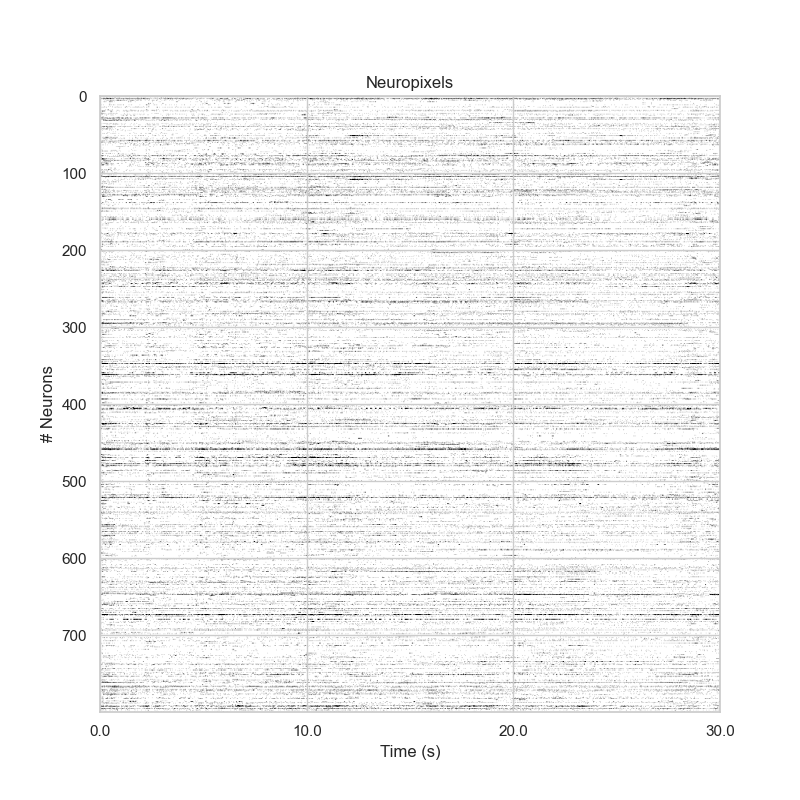
\includegraphics[width=0.6\textwidth]{neuropixels.png}
    \caption{Neural Responses}
    \label{fig:neuropixels}
\end{figure}

We then decided to visualize different dimensionality reductions of the neural responses to see if there is any clear clustering. We began with PCA and then moved on to t-SNE. For PCA we used the top $3$ dimensions and each point is colored based on the corresponding frame ID. 

\begin{figure}[H]
    \centering
    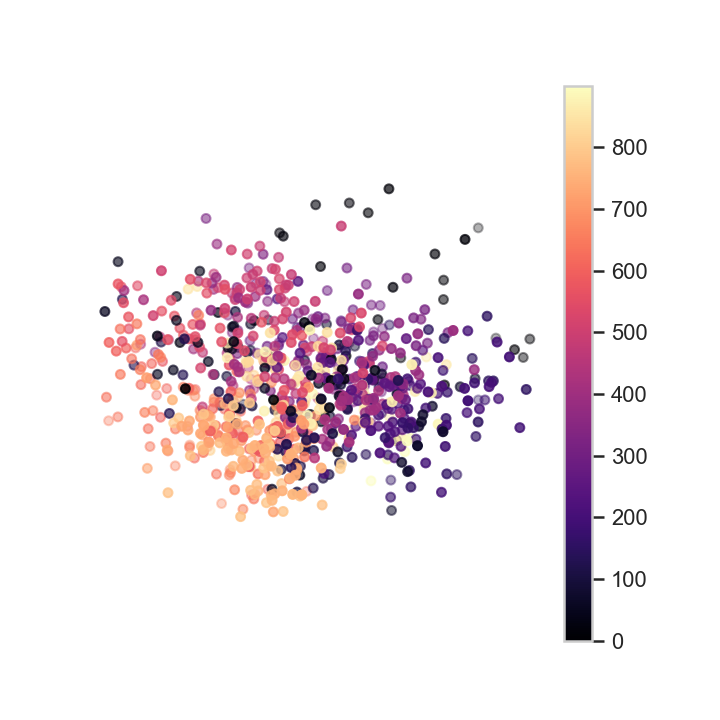
\includegraphics[width=0.5\textwidth]{3d_pca_neuropixels.png}
    \caption{3 dimensional PCA of Neuropixels}
    \label{fig:3d_pca_neuropixels}
\end{figure}

We can see that the PCA plot shows some clustering based on the frame ID but it does not show clear separation between the PCA components for individual frame IDs which would make it difficult to classify. We also plotted the explained variance of the PCA components.

\begin{figure}[H]
    \centering
    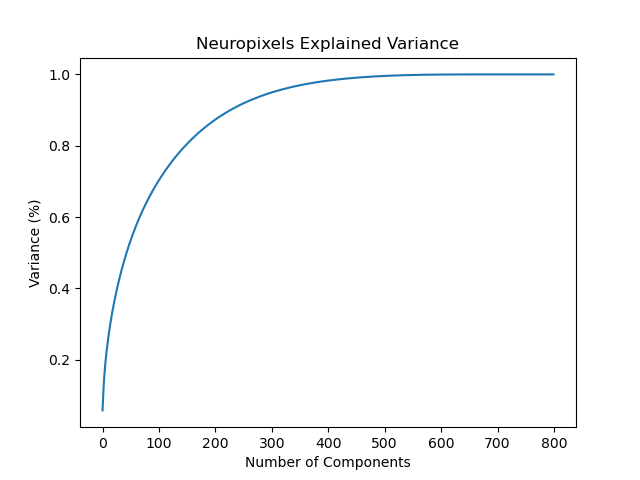
\includegraphics[width=0.5\textwidth]{neuropixels_pca_explained_variance.png}
    \caption{Explained Variance of PCA Components}
    \label{fig:explained_variance_pca}
\end{figure}

From the plot we can see that with around $200$ PCA components we are able to capture $90\%$ of the variance across samples which is only a quarter of the full $800$ neuropixels. We then used $2$ dimensional t-SNE to visualize the neural responses. 

\begin{figure}[H]
    \centering
    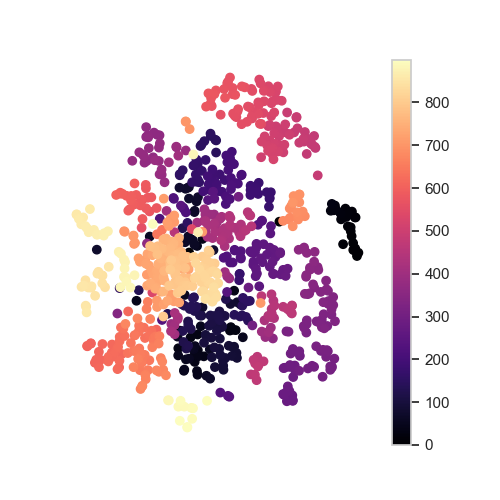
\includegraphics[width=0.5\textwidth]{tsne_neuropixels.png}
    \caption{2 dimensional t-SNE of Neuropixels}
    \label{fig:2d_tsne_neuropixels}
\end{figure}

The t-SNE plot showed some clustering based on the frame ID but there was still was not clear separation between the individual frames. From these plots we can gather that simple dimensionality reduction tools with a classifier like logistic regression or KNN may not be able to accurately predict the frame ID based on the neural responses. 

\subsection{Data Preprocessing}
\label{subsec:data_preprocessing}
In the first step of preprocessing the data we needed to reduce the time dimension for each neuropixel such that the number of stimulus or samples is equal to the number of frames. We did this by taking groups of $4$ bins and then computing the average of the bins in the group. This reduced the number of bins from $3600$ to $900$ per presentation. So in total we had $9000$ samples rather than $36000$ samples. Next we looked into individual neuropixels. For some neuropixels there activations were $0$ for all frames during a single presentation so we decided to remove those neuropixels. This reduced the number of neuropixels from $800$ to $772$. 

\subsection{Neuropixel Decoding}
\label{subsec:neuropixel_decoding}
We investigated starting from the $772$ neuropixels the decoding $R^2$ score for frame ID using a simple linear regression model. We used $9$ of the stimulus presentations for training and withheld $1$ presentation for test set. We fit a Lasso regression model with alpha, the regularization parameter, set to $0.08$. 
\begin{figure}[H]
    \centering
    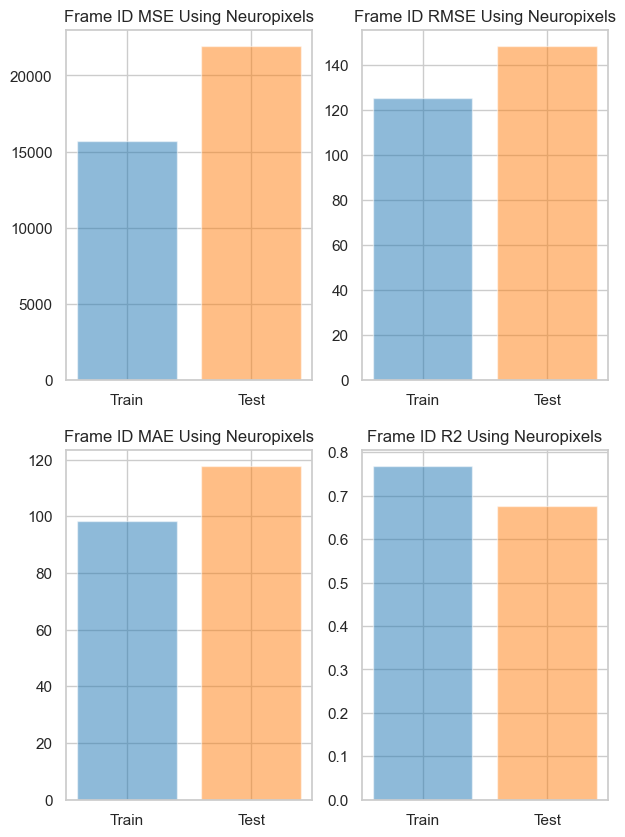
\includegraphics[width=0.5\textwidth]{frame_id_metrics_lasso_.08.png}
    \caption{Lasso Regression Frame ID Decoding}
    \label{fig:lasso_frame_id}
\end{figure}
We can see that there is a high $R^2$ score for the frame ID decoding using the Lasso regression model with the full set of neuropixels used as features. However, the MAE and RMSE are both quite high which could be indicative that the even though the neuropixels are capturing a significant amount of variance across the frames it isn't enough to accurately predict individual frame IDs. Following the results we were interested in seeing how well the neuropixel features would perform with logistic regression. We used the same training and test set as before and fit a logistic regression model.

\begin{figure}[H]
    \centering
    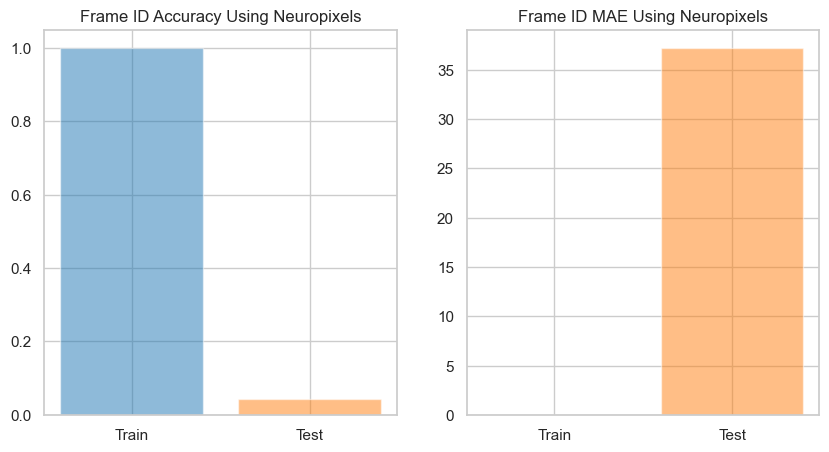
\includegraphics[width=0.7\textwidth]{frame_id_metrics_logistic.png}
    \caption{Train and Test Accuracy and MAE of Logistic Regression Frame ID Decoding}
    \label{fig:neuropixel_logistic_frame_id}
\end{figure}

We can see from the figure that there is high overfitting as the training accuracy is around $1$ but the test accuracy is only $0.04$. We can also see that the overall MAE or average frame difference is also much higher in the test set compared to the training set. In an attempt to reduce the overfitting we tried tuning the $C$ or inverse regularization term for logistic regression but the train accuracy was still very high with approximately the same MAE. Finally we translated the predicted frame IDs into its corresponding images. Below shows the first $10$ predicted frame IDs and corresponding frames on the test set using logistic regression.

\begin{figure}[H]
    \centering
    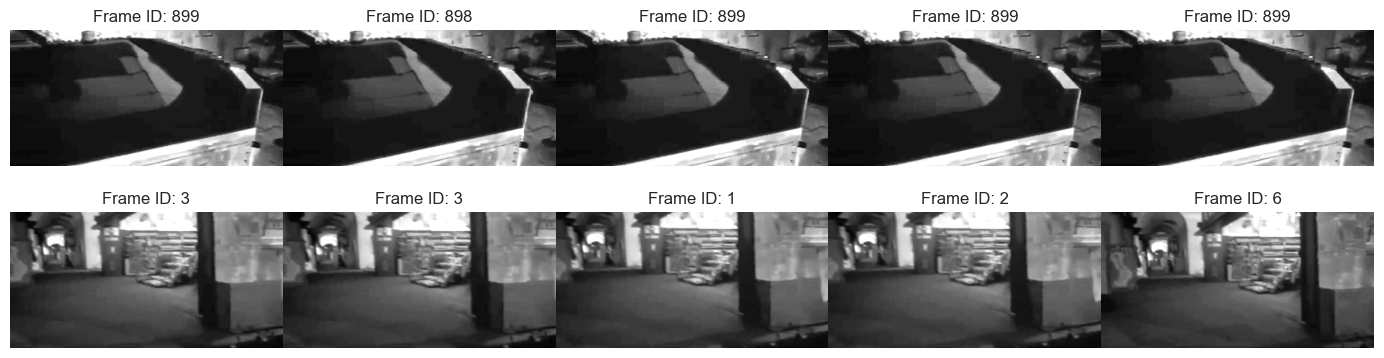
\includegraphics[width=0.8\textwidth]{neuropixel_logistic_reg_video.png}
    \caption{Logistic Regression Decoded Frames}
    \label{fig:neuropixel_logistic_frame_id_decoded}
\end{figure}

We can see that the model predicted the last frame ID for $4$ out of the first $5$ decoded frames and then the following $5$ frames while actually being different frame IDs visually are very similar. This could explain why the decoding accuracy is so poor. The neuronpixels will most likely respond the same way to very similar frames especially in the lower level visual cortex.

\subsection{PCA Decoding}
\label{subsec:pca_decoding}
Generall neural responses can be very noisy so we were curious if first reducing the dimensionality of the neural responses and then fitting a Lasso or Logistic regression model would improve the frame ID decoding. Initially we wanted to see if fitting a Lasso regression model with $3$ PCA components and an alpha of $0.08$ would achieve similar $R^2$ scores as using the full set of neural responses.

\begin{figure}[H]
    \centering
    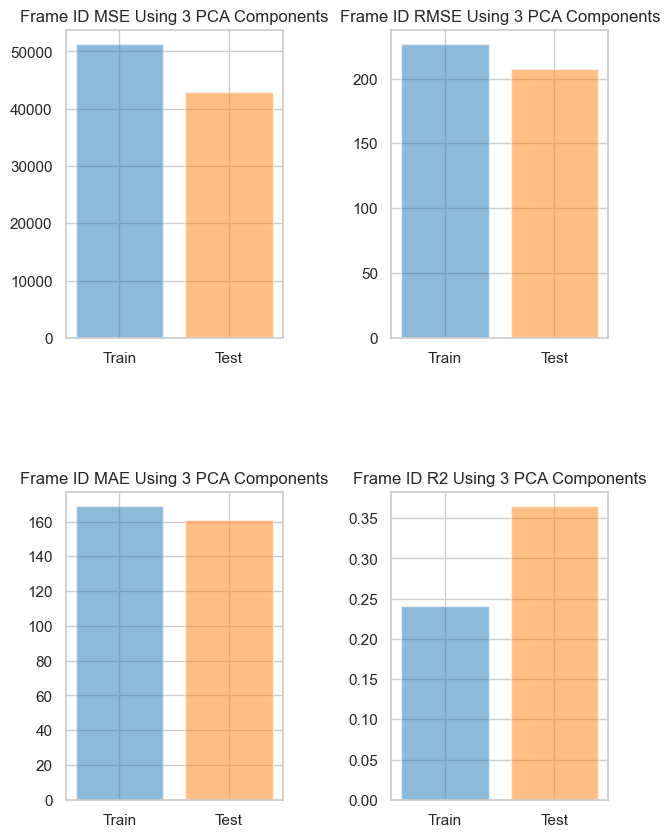
\includegraphics[width=0.5\textwidth]{frame_id_metrics_lasso_using_pca.08.png}
    \caption{Lasso Regression Frame ID Decoding with 3 PCA Components}
    \label{fig:pca_frame_id_lasso}
\end{figure}

We can see that the $R^2$ score is much lower than the full set of neuropixels but the MAE and RMSE are actually very similar to the full set of neuropixels. Our initial thought was that $3$ PCA components may not account for enough of the variance so before we fit a logistic regression model we decided to find the most optimal number of PCA components using a grid search with $7$ training presentations and $2$ validation presentations. Here are the results of the grid search.

\begin{figure}[H]
    \centering
    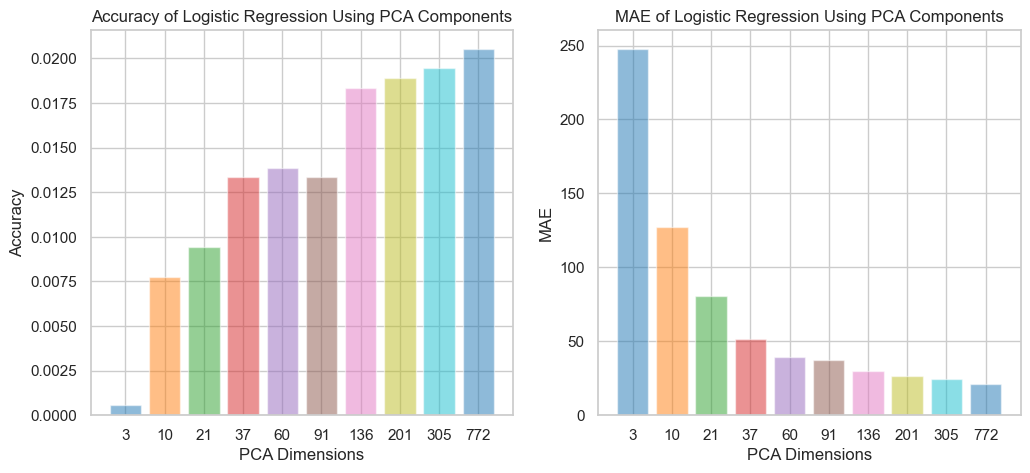
\includegraphics[width=0.7\textwidth]{logistic_pca_accuracy_mae.png}
    \caption{Grid Search for PCA Components in Logistic Regression Frame ID Decoding}
    \label{fig:logistic_pca_accuracy_mae}
\end{figure}

We can see that the highest accuracy is still while using the full $772$ dimensions but we also noticed that even with half as many PCA components we are able to achieve a comparable MAE and accuracy to using the full set of neuropixels. According to the PCA explained variance curve with $305$ dimensions we are able to capture $90\%$ of the variance across samples. We decided to use the $305$ PCA components and fit a logistic regression model with $C$ value of $.4$ on the $9$ training presentations and were able to see the following train and test accuracy and MAE.

\begin{figure}[H]
    \centering
    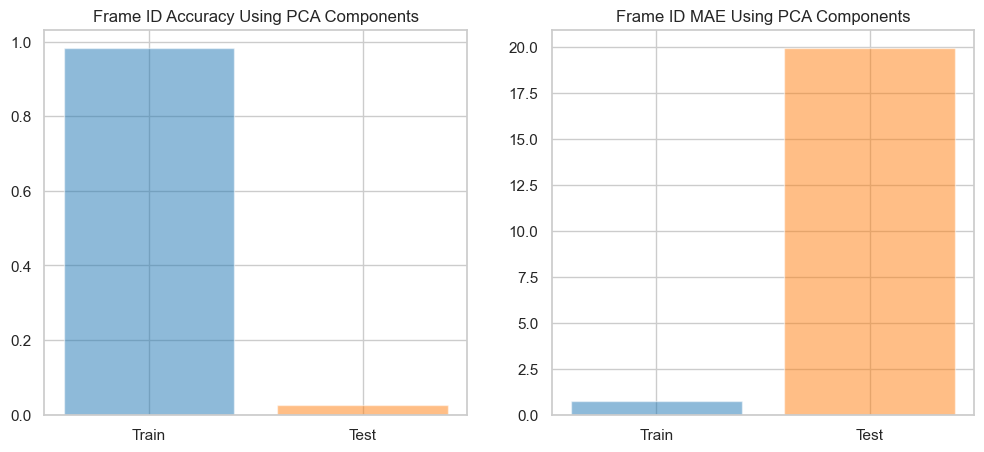
\includegraphics[width=0.7\textwidth]{frame_id_metrics_logistic_C_.4_pca.png}
    \caption{Train and Test Accuracy and MAE of Logistic Regression Frame ID Decoding with PCA Components}
    \label{fig:logistic_pca_frame_id}
\end{figure}

Similar to the full set of neuropixels, \hyperref[fig:neuropixel_logistic_frame_id]{Figure~\ref{fig:neuropixel_logistic_frame_id}}, we can see that there is a high overfitting in the model since the training accuracy is at $1$ but the test accuracy is at $.02$ even after applying at $C$ value of $.4$. Notably, while the accuracy is lower than the full set of neuropixels the MAE is actually lower when using the $305$ PCA components. Here are the first $10$ predicted frame IDs on the test set using the logistic regression model fit on $305$ PCA components.

\begin{figure}[H]
    \centering
    \includegraphics[width=0.8\textwidth]{.9_pca_logistic_reg_video.png}
    \caption{Logistic Regression Decoded Frames with .9 Explained Variance PCA Components}
    \label{fig:pca_logistic_frame_id_decoded}
\end{figure}

We can see that the logistic regression model using PCA components is no longer predicting very high frame IDs within the first $10$ frames which was the case for the full set of neuropixels shown in \hyperref[fig:neuropixel_logistic_frame_id_decoded]{Figure~\ref{fig:neuropixel_logistic_frame_id_decoded}}. The decoded frames however are still not varied in this case the frame ID $0$ was actually predicted $4$ times. In addition, similar conclusions can be drawn that the decoded frames, despite being different frame IDs, the actual contents of each frame are very similar visually.

\subsection{VAE Reconstruction and Decoding}
\label{subsec:vae_reconstruction_and_decoding}
After exploring some basic classifiers to decode from neural responses to the Frame ID and from PCA components to Frame ID we decided to train a VAE model to reconstruct the neural responses and see if the learned latents could have a better decoding performance for frame ID. We also tested out using different forms of guidance for the VAE model. We tested using no guidance on the latents, a separate head to predict frame ID, and a separate head to predict the PCA components of the DINO embeddings. We trained the VAE model for $200$ epochs and used a beta value on the KL divergence of $0.05$ annealed over the $200$ epochs which we found to be the best in terms of validation reconstruction $R^2$ score. We also found that the best model architecture was using $3$ hidden layers in the encoder with LeakyReLU activations and $2$ hidden layers in the decoder. 
For the size of the latent space we used $128$ dimensions the reasoning was mostly to have a valid comparison with the CEBRA \cite{schneider2023} latents which also used $128$ dimensions. For the loss function in order to penalize poor reconstruction we measured the MSE loss between the reconstructed neural responses and the true neural responses in addition to the KL divergence loss. When training the VAE model with guidance on the latents we added an additional loss term that penalized the MSE loss between the predicted DINO embeddings and the true DINO embeddings or cross-entropy loss between the predicted frame ID and the true frame ID. In order to quantify reconstruction performance both for neural responses and for the DINO embeddings we used the $R^2$ score on the train and validation set. We also measured the accuracy and MAE for the frame ID prediction.
We mention using guidance for some of the VAE models. By guidance we mean adding a supervised head to the VAE model that predicts the DINO embeddings or the frame ID. This head is a torch linear layer that maps from the latent space to the DINO embeddings or frame ID. By adding supervision to the latent space we are able to guide the model to learn a latent space that hopefully encodes both information about the neural responses and more information about the actual frames presented in the stimulus.

\subsubsection{VAE No Guidance}
\label{subsubsec:vae_no_guidance}
The following are the results of the VAE model with no guidance on the latents. We measured the model's neural reconstruction $R^2$ score on a train set of $7$ presentations and a validation set of $2$ presentations.

\begin{figure}[H]
    \centering
    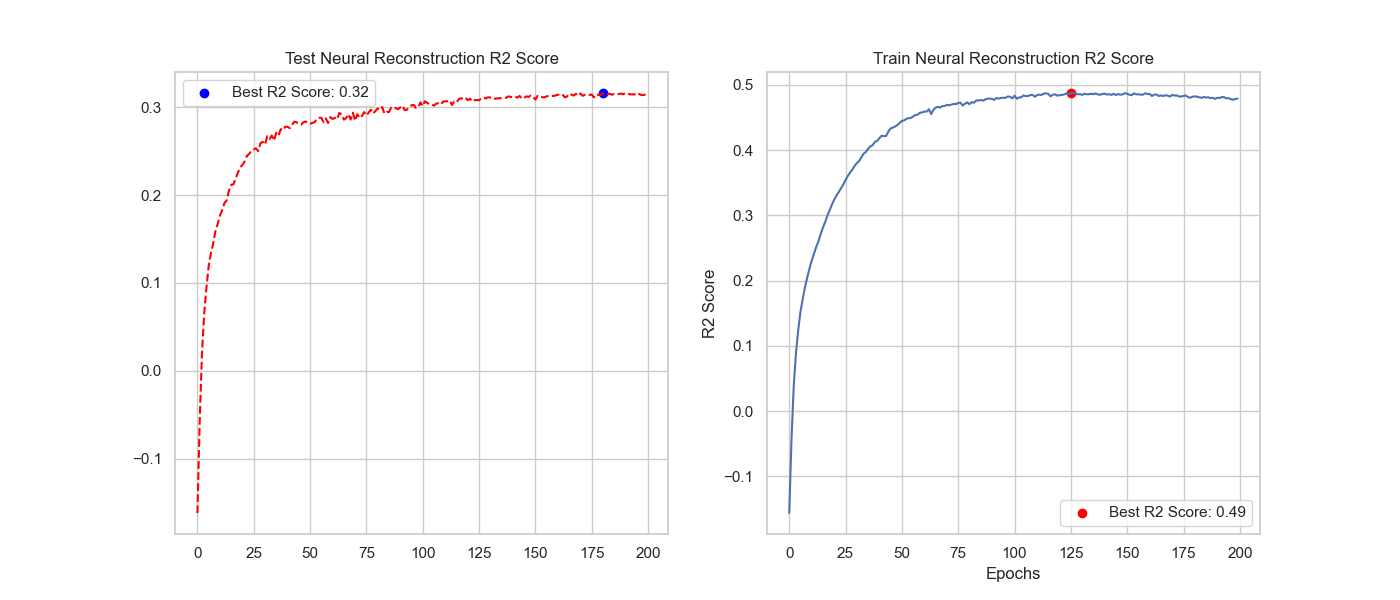
\includegraphics[width=1.0\textwidth]{x_r2_128dim_200_epochs_0.05beta_2_layer.png}
    \caption{VAE No Guidance Reconstruction $R^2$ Score}
    \label{fig:vae_no_guidance}
\end{figure}

We can see from the figure above that the model has a decent reconstruction score on the validation set for the full set of $772$ neuropixels. The model is able to capture around $30\%$ of the variance in the neural responses. In an effort to improve the reconstruction performance we were curious if taking the neuropixels with the highest variance across stimulus presentations would reduce noise and improve the $R^2$ score. First we took the top $393$ neuropixels with the highest variance because by using the covariance matrix we were able to measure that with $393$ neuropixels we could explain approximately $90\%$ of the variance across all stimulus. Specifically, we calculated explained variance by taking the $tr(\Sigma_{features})$ where $\Sigma_{features}$ is the covariance matrix of the top $393$ neuropixels and dividing it by $tr(\Sigma_{full})$ where $\Sigma_{full}$ is the covariance matrix of the full set of $772$ neuropixels. 

\begin{figure}[H]
    \centering
    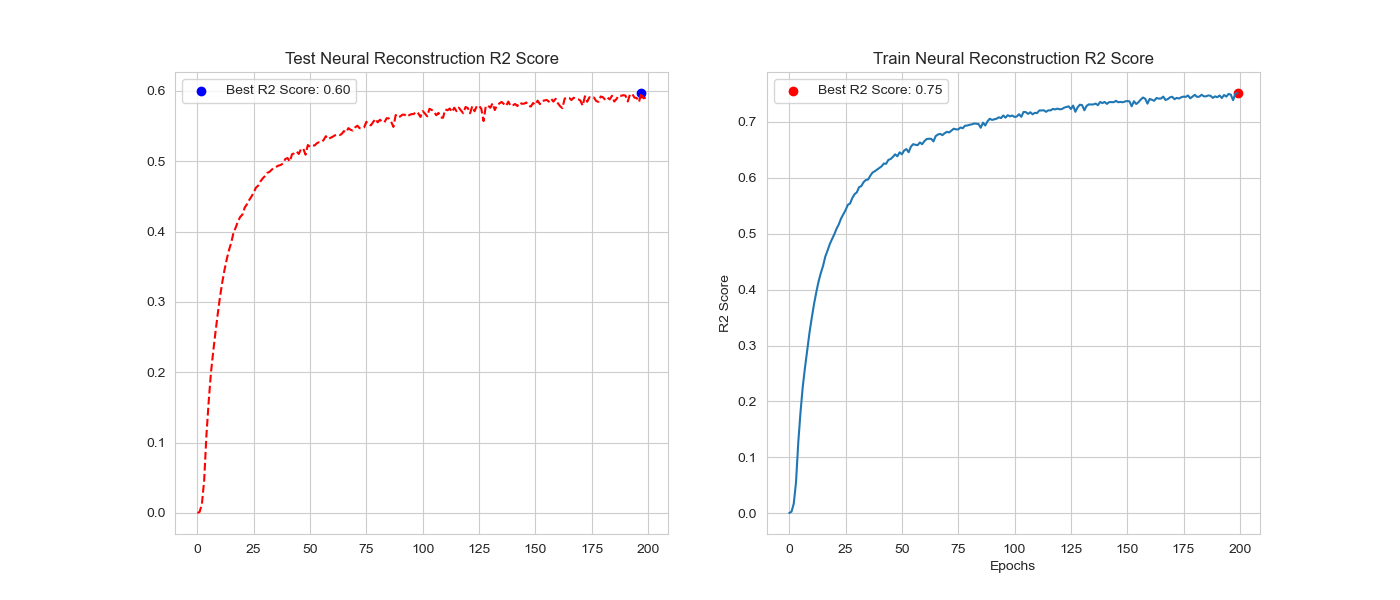
\includegraphics[width=1.0\textwidth]{x_r2_128dim_393_top_var_200_epochs_0.05_beta_2_layer.png}
    \caption{VAE No Guidance Reconstruction $R^2$ Score with Top 393 Neuropixels}
    \label{fig:vae_no_guidance_top393}
\end{figure}

As expected we see that the $R^2$ score is higher when using the top $393$ neuropixels compared to the full set of $772$ neuropixels. Of course the could be attributed to the fact that it is easier for a model to learn a reconstruction when the input has less dimensions but from the PCA exploration in \hyperref[fig:explained_variance_pca]{Figure~\ref{fig:explained_variance_pca}} of the data one alternative hypothesis is that there might be some neuropixels that are not actually encoding information about the stimulus which would add noise to our reconstructions making the $R^2$ score lower. We also explored what the reconstruction performance would be if we use the top $503$ neuropixels which using the same calculations we measured to capture $95\%$ of the variance across the stimulus.

\begin{figure}[H]
    \centering
    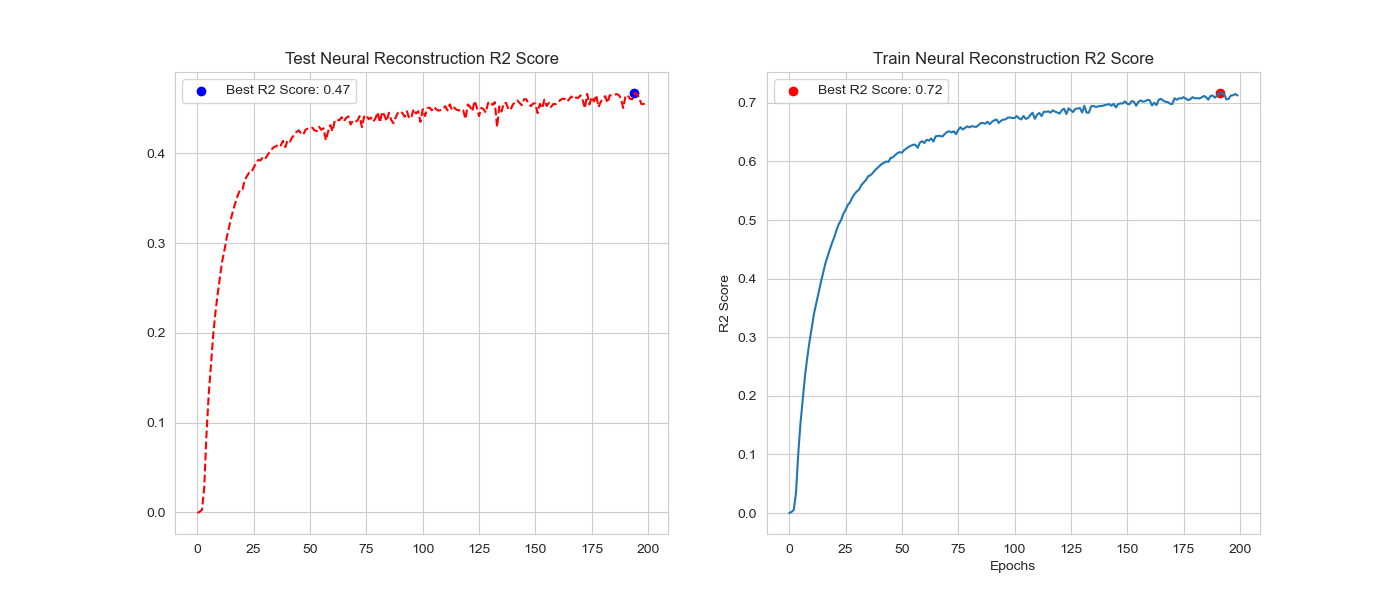
\includegraphics[width=1.0\textwidth]{x_r2_128dim_503_top_var_200_epochs_0.05_beta_2_layer.png}
    \caption{VAE No Guidance Reconstruction $R^2$ Score with Top 503 Neuropixels}
    \label{fig:vae_no_guidance_top503}
\end{figure}

The validation set reconstruction performance using $503$ neuropixels with the highest variance across stimulus is noticeably lower than with the top $393$ neuropixels but still significantly better than the full set of $772$ neuropixels. 

\subsubsection{VAE Guidance using DINO Embeddings}
\label{subsubsec:vae_guidance_DINO}
The following are the results of the VAE model with DINO embeddings acting as guidance on the latent space. DINO which stands for distillation with no labels are low dimensional embeddings that can capture semantically meaningful information about images \cite{dino}. In our case we were provided DINO \cite{dino} embeddings for each of the video frames. These embeddings are used by the CEBRA model to determine the positive and negative samples for contrastive learning \cite{schneider2023}.

We measured the model's neural reconstruction $R^2$ score on a train set of $7$ presentations and a validation set of $2$ presentations. We also measured the model's DINO \cite{dino} embedding $R^2$ score on the same train and validation set. Initially we used the entire DINO \cite{dino} embedding as guidance which had $768$ dimensions. During training however we noticed the model's train and validation reconstruction of the embedding stayed in the negatives. We then decided to use PCA to reduce the DINO \cite{dino} embeddings from $768$ dimensions to $32$ dimensions. The $32$ dimensions were able to capture $90\%$ of the variance across DINO \cite{dino} embedding samples. Here are the neural reconstruction results of the VAE model with guidance using the PCA of DINO \cite{dino} embeddings after selecting the top $503$ neuropixels based on variance.

\begin{figure}[H]
    \centering
    \includegraphics[width=1.0\textwidth]{x_r2_128dim_503_top_var_200_epochs_0.05_beta_2_layer_.9_pca_DINO_embed.png}
    \caption{$503$ Neuropixel Neural Reconstruction $R^2$ Score}
    \label{fig:vae_guidance_DINO_pca}
\end{figure}

Comparing the reconstruction performance with VAE using no guidance on the top $503$ neuropixels, \hyperref[fig:vae_no_guidance_top503]{Figure~\ref{fig:vae_no_guidance_top503}}, we can see that the model with guidance on the DINO \cite{dino} embeddings has a slightly lower reconstruction performance on validation with the best $R^2$ score at $.47$ with no guidance and $.44$ with guidance. Next we wanted to see how well the model was able to reconstruct the DINO \cite{dino} embeddings.

\begin{figure}[H]
    \centering
    \includegraphics[width=.9\textwidth]{.9_pca_DINO_embed_r2_128dim_503_top_var_200_epochs_0.05_beta_2_layer.png}
    \caption{Reconstruction of $32$ Dimension PCA of DINO Embedding $R^2$ Score}
    \label{fig:vae_guidance_DINO_pca_DINO_embed_r2}
\end{figure}

Above we plotted the DINO \cite{dino} embedding $R^2$ score for the validation and training sets starting at epoch $50$ in the training process. The reason is because the DINO \cite{dino} embedding $R^2$ score was negative at the beginning of training. We can see that the model was able to learn to capture some of the variance between DINO \cite{dino} embeddings with the best $R^2$ score at $.19$ on the validation set and $.23$ on the training set.

We define beta as the hyperparameter multiplied to the KL divergence term before adding it to the total loss. Since we kept the same beta value of $.05$ for the KL divergence loss above we wanted to see how well the model would do with a lower beta value. The KL divergence loss acts as a regularizer on the latent space and a lower beta value would mean that the model would be less penalized for deviating from the prior distribution. In order to learn to map from latents to a complex embedding we may need to loosen the constraints imposed by the KL divergence term. With that in mind we tried a beta value of $.008$ for the KL divergence loss and annealed it over $200$ epochs.

\begin{figure}[H]
    \centering
    \includegraphics[width=1.0\textwidth]{x_r2_128dim_503_top_var_200_epochs_0.008_beta_2_layer_.9_pca_DINO_embed.png}
    \caption{$503$ Neuropixel Neural Reconstruction $R^2$ Score Using .008 Beta}
    \label{fig:vae_guidance_DINO_pca_neural_reconstruction_.008_beta}
\end{figure}

From the figure above the model performed slightly worse on the neural reconstruction with a peak $R^2$ score of $.34$ on the validation set compared to the model with a beta value of $.05$ which showed a peak neural reconstruction $R^2$ score of $.44$, \hyperref[fig:vae_guidance_DINO_pca]{Figure~\ref{fig:vae_guidance_DINO_pca}}. This was expected since the KL divergence loss with a higher beta value would help the model to generalize better to unseen data. We also plotted the DINO \cite{dino} embedding $R^2$ score for the validation and training sets.

\begin{figure}[H]
    \phantomsection  % Create an invisible anchor here
    \centering
    \includegraphics[width=.9\textwidth]{.9_pca_DINO_embed_r2_128dim_503_top_var_200_epochs_0.008_beta_2_layer.png}
    \caption{Reconstruction of $32$ Dimension PCA of DINO Embedding $R^2$ Score Using .008 Beta}
    \label{fig:vae_guidance_DINO_pca_DINO_embed_r2_.008_beta}
\end{figure}

The lower beta value however did allow the model to learn a latent space that was able to better capture the variance in the DINO \cite{dino} embeddings. We were able to see higher reconstruction performance of DINO \cite{dino} embeddings when using a beta value of $.008$ than $.05$. From the figure above the best $R^2$ score on the validation set was $.59$ which was higher than the VAE model trained with beta of $.05$ which peaked at $.19$, \hyperref[fig:vae_guidance_DINO_pca_DINO_embed_r2]{Figure~\ref{fig:vae_guidance_DINO_pca_DINO_embed_r2}}. 

We also wanted to see how well the model was able to perform on the full set of neuropixels. Instead of using the top $503$ neuropixels we used the full set of $772$ neuropixels and used a beta value of $.008$ for the KL divergence loss annealed over $200$ epochs. Something to note is that this same combination without guidance had very poor neural reconstruction performance. 

\begin{figure}[H]
    \centering
    \includegraphics[width=1.0\textwidth]{x_r2_128dim_772_top_var_200_epochs_0.008_beta_2_layer_.9_pca_DINO_embed.png}
    \caption{Neural Reconstruction $R^2$ Score with Full Set of Neuropixels}
    \label{fig:vae_guidance_DINO_pca_full_neuropixels}
\end{figure}

Surprisingly, the model with guidance on the DINO \cite{dino} embeddings was able to achieve a higher neural reconstruction $R^2$ score compared to the model with no guidance. Initially we had trained a VAE model with no guidance and a beta value of $.008$ to learn the reconstruction of the full set of $772$ neuropixels the model had a peak $R^2$ score of $.18$ on the validation set and the validation $R^2$ slowly became negative over the course of training. On the other hand the model with guidance on the DINO \cite{dino} embeddings has a peak $R^2$ score of $.20$ but we did not see the $R^2$ score become negative over the course of training except for one sharp drop towards the end of training. Below we also plotted the $R^2$ score for the reconstructed $32$ dimension PCA components of the DINO \cite{dino} embeddings on the validation and training sets.

\begin{figure}[H]
    \centering
    \includegraphics[width=.9\textwidth]{.9_pca_DINO_embed_r2_128dim_772_top_var_200_epochs_0.008_beta_2_layer.png}
    \caption{Reconstruction of $32$ Dimension PCA of DINO Embedding $R^2$ Score with Full Set of Neuropixels}
    \label{fig:vae_guidance_DINO_pca_DINO_embed_r2_full_neuropixels}
\end{figure}

We can see that the model was able to achieve a similarly high $R^2$ score on the DINO \cite{dino} embeddings when using the full set of neuropixels compared to the top $503$ neuropixels. 

\subsubsection{VAE Guidance using Frame ID}
\label{subsubsec:vae_guidance_frame_id}
We also attempted to directly use the frame ID as guidance for the VAE model. Using a linear layer we mapped from the $128$ dimensions of the latent space to a $900$ dimensional vector which was then used in torch's cross-entropy loss. The cross-entropy loss term was added to the total loss which consisted of mse loss between the reconstruction neural response and true neural response and the KL divergence. The predictions from this layer for the frame ID would just be the argmax from the $900$ dimension vector. We also kept the same beta value of $.05$ for the KL divergence loss and annealed it over $200$ epochs and used the $503$ top variance neuropixels which in theory should reduce the noise in the neural responses.

Below are the training and validation set results of the VAE model with guidance using the frame ID on the top $503$ neuropixels based on variance using a beta value of $.05$ for the KL divergence loss.

\begin{figure}[H]
    \centering
    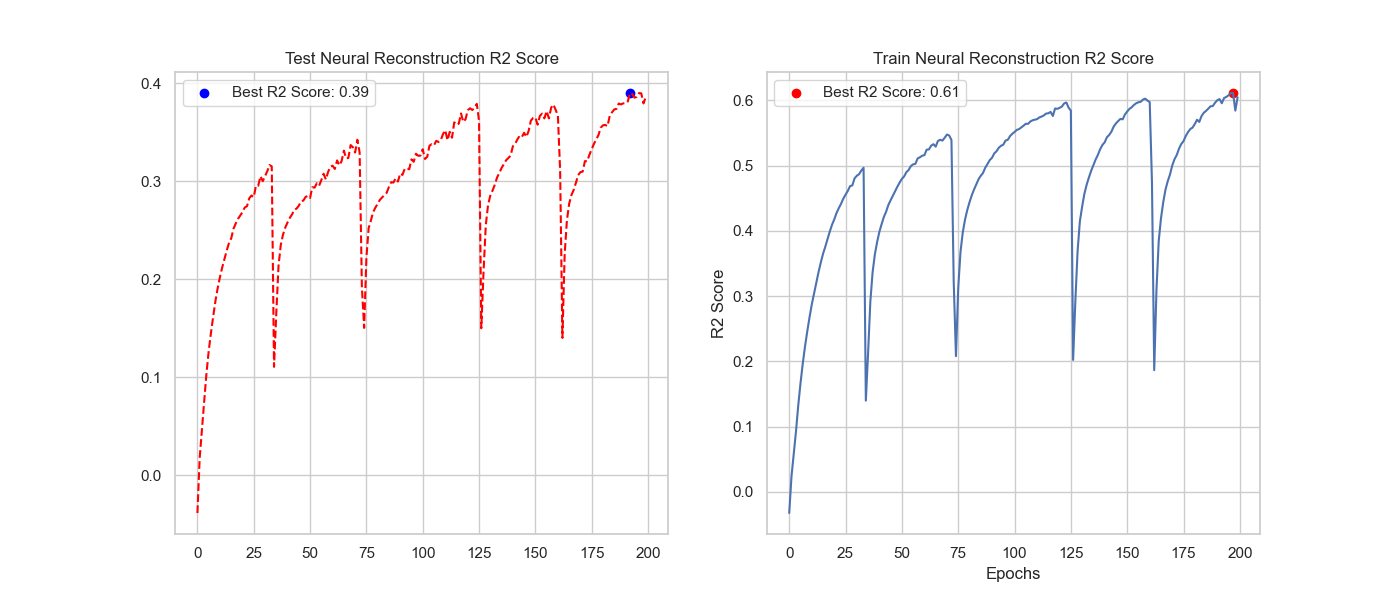
\includegraphics[width=1.0\textwidth]{x_r2_128dim_503_top_var_200_epochs_0.05_beta_2_layer_frame_id_guidance.png}
    \caption{VAE Guidance using Frame ID $503$ Neuropixel Neural Reconstruction $R^2$ Score}
    \label{fig:vae_guidance_frame_id}
\end{figure}

The model using frame ID shows lower $R^2$ scores for neural reconstruction compared to the model with guidance on the DINO \cite{dino} embeddings and using the same beta value of $.05$, see \hyperref[fig:vae_guidance_DINO_pca]{Figure~\ref{fig:vae_guidance_DINO_pca}}, and lower than when using no guidance, see \hyperref[fig:vae_no_guidance_top503]{Figure~\ref{fig:vae_no_guidance_top503}}. We can see that during the training process there are sharp drops in the training and validation $R^2$ scores which we did not see in the other models. We also explored the accuracy of the frame ID prediction on the train and validation sets.

\begin{figure}[H]
    \centering
    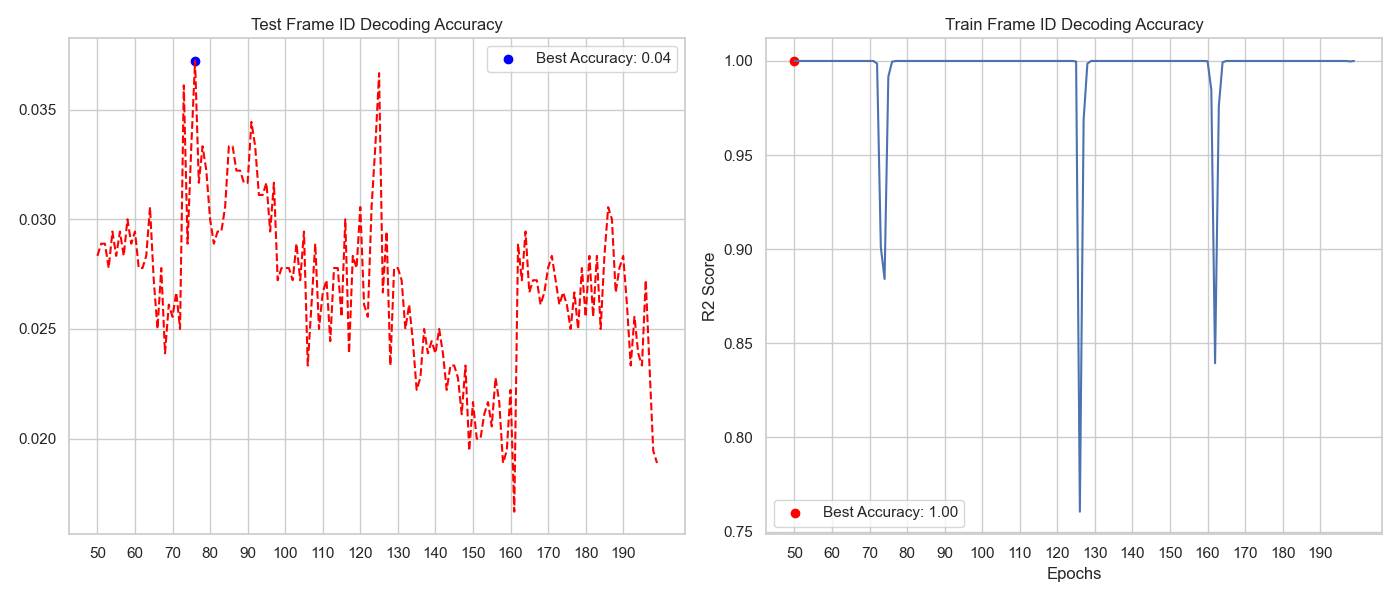
\includegraphics[width=1.0\textwidth]{frame_id_accuracy_128dim_503_top_var_200_epochs_0.05_beta_2_layer.png}
    \caption{VAE Guidance using Frame ID Frame ID Prediction Accuracy}
    \label{fig:vae_guidance_frame_id_accuracy}
\end{figure}

The training accuracy above is around $1$ for most of the training but the validation set accuracy peaks early at around $.04$ and then begins to drop. This is indicative of the model overfitting to the training data so we decided to try adding a dropout layer with a rate of $.2$ in the classification head which is the linear layer mapping from the latent space to the frame ID. 

\begin{figure}[H]
    \centering
    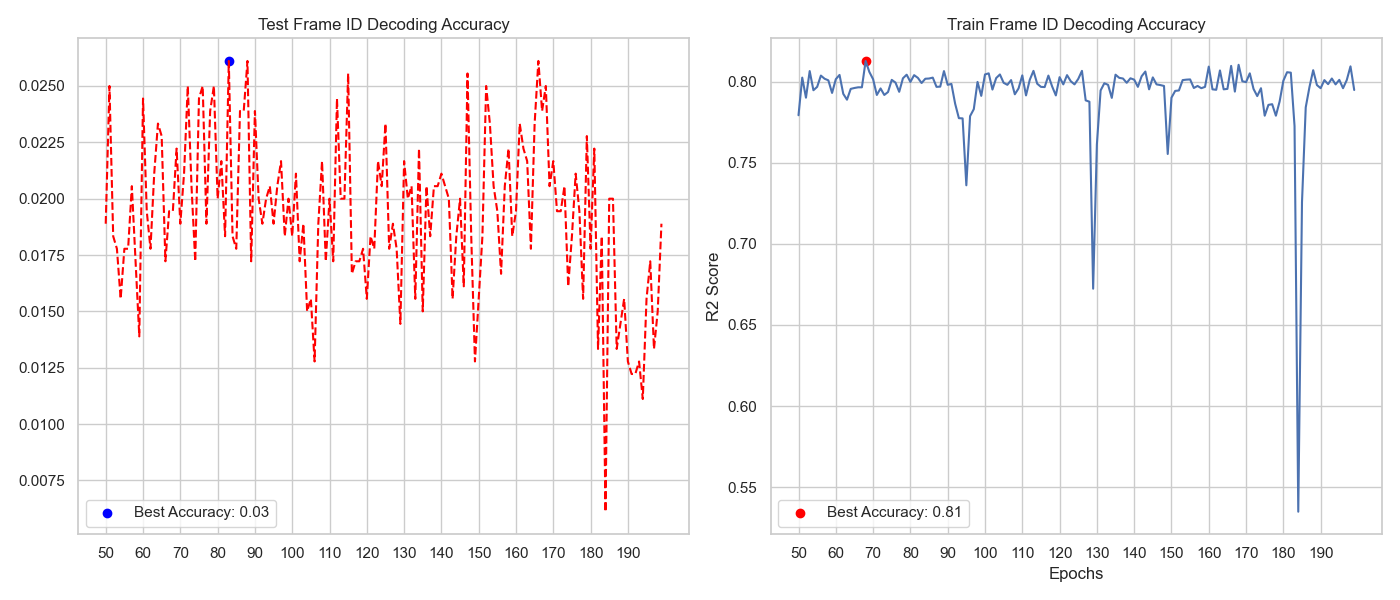
\includegraphics[width=1.0\textwidth]{frame_id_accuracy_128dim_503_top_var_200_epochs_0.05_beta_2_layer_.2_dropout.png}
    \caption{VAE Guidance using Frame ID Frame ID Prediction Accuracy with .2 Dropout}
    \label{fig:vae_guidance_frame_id_accuracy_dropout}
\end{figure}

The dropout layer did not seem to improve the model's validation set peak accuracy but it did reduce the training accuracy. One potential explanation for the model's poor performance when using frame ID as guidance is that the frame ID is not actually encoded in the neural responses. Since many frames that are close in time are very similar it is possible that a region like V1 would not be able to differentiate between the frames. 

We also explored using the full set of $772$ neuropixels with guidance on the frame ID and using smaller beta values for the KL divergence loss which showed significant performance benefits when training with the DINO embeddings as guidance. However, the model with frame ID as guidance did not show any improvements when using a lower beta value for the KL divergence loss or when using the full set of $772$ neuropixels.

\subsubsection{VAE Frame ID Decoding Results}
\label{subsubsec:vae_frame_id_decoding}
Previously during VAE model hyperparameter tuning we were using $7$ training and $2$ validation sets of stimulus presentations where each presentation consisted of $900$ frames of a video. Now with the held out test set we wanted to compare how well each of the latents learned by the VAE models are able to decode the frame ID based on accuracy and MAE. We used a logistic regression model to decode the frame ID from the latents and we also tried using KNN with the number of neighbors parameters set to $2$ to decode the frame ID. The number of neighbor parameters was chosen using grid search on the train and validation presentations with $2$ having the lowest MAE and highest accuracy. As a recap we trained the following different VAE models over $200$ epochs and stored their learned latents. 

\begin{itemize}
    \item VAE No Guidance ($503$ Top Neuropixels)
    \item VAE Guidance using DINO Embeddings ($503$ Top Neuropixels)
    \item VAE Guidance using Frame ID ($503$ Top Neuropixels)
    \item VAE Guidance using DINO Embeddings with .008 Beta ($503$ Top Neuropixels)
    \item VAE Guidance using DINO Embeddings with .008 Beta (All Neuropixels)
\end{itemize}

\begin{figure}[H]
    \centering
    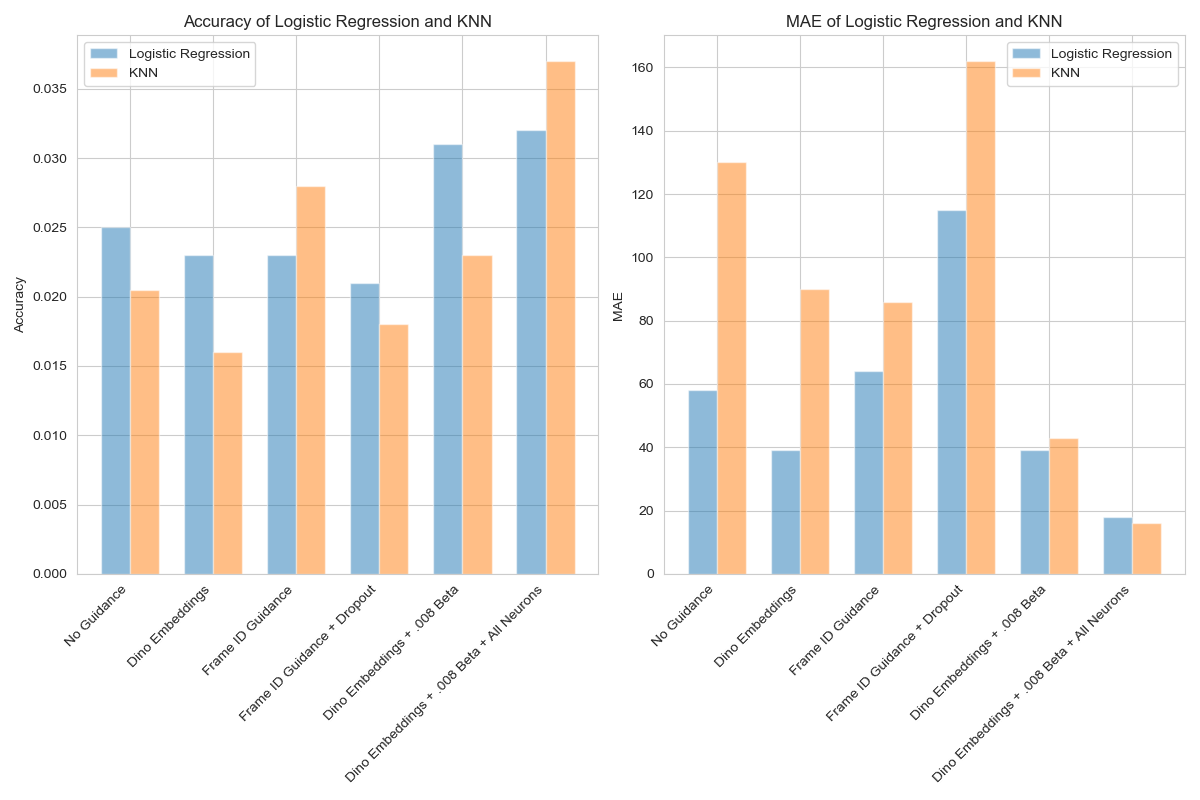
\includegraphics[width=1.0\textwidth]{vae_models_logistic_knn_comparison.png}
    \caption{VAE Frame ID Decoding Accuracy and MAE Comparison}
    \label{fig:vae_frame_id_decoding_comparison}
\end{figure}

For models such as \textit{VAE No Guidance} and \textit{VAE Guidance using Frame ID} we decided to only show the top $503$ neuropixels based on variance performance on the test set because the latents learned to reconstruct the full set of $772$ neuropixels did not show any significant performance benefits. On the other hand for models such as VAE Guidance using DINO Embeddings with .008 Beta we are showing the full set of $772$ neuropixels because the latents learned to reconstruct the full set of $772$ neuropixels showed significant performance improvements.

We can see that in the comparison between KNN and Logistic regression the logistic regression model was generally able to perform better with higher accuracy and lower MAE but out of the $6$ models that we tested the highest accuracy and lowest MAE was achieved using KNN. By a significant margin, the VAE model with guidance on the latents to learn the DINO \cite{dino} embeddings had the highest accuracy and lowest MAE. Specifically, using the full $772$ neuropixels and a annealed beta value of $.008$ we were able to achieve the highest accuracy of around $.04$ and the lowest MAE at $16$. If we compare these results to using the $503$ top variance neuropixels with logistic regression which had an accuracy of $.025$ and MAE of $58$ we can see that the VAE model with guidance on the latents was able to perform better. The tradeoff is that with guidance the neural reconstruction performance was lower than without guidance, comparing \hyperref[fig:vae_no_guidance]{Figure~\ref{fig:vae_no_guidance}} and \hyperref[fig:vae_guidance_DINO_pca_full_neuropixels]{Figure~\ref{fig:vae_guidance_DINO_pca_full_neuropixels}}. These findings were definitely unexpected since originally we believed that directly using frame ID as guidance would be the best way to supervise the latents to encode information about the individual frames. However, DINO \cite{dino} embeddings may actually encode more semantic information about what the stimulus is showing compared to just an index of the frame. Finally below we are showing the first $10$ predicted frame IDs using a KNN classifier on the latents of the best performing model, $32$ component PCA of the DINO \cite{dino} embeddings as guidance with a beta value of $.008$ and using the full set of $772$ neuropixels.

\begin{figure}[H]
    \centering
    \includegraphics[width=1.0\textwidth]{772_vae_hidden_.9_pca_DINO_knn_video.png}
    \caption{Predicted Frame IDs by VAE latents guided by PCA of DINO Embeddings}
    \label{fig:vae_frame_id_decoded_video}
\end{figure}

\subsection{CEBRA Reproduction}
\label{subsec:cebra_reproduction}
The CEBRA API \cite{cebra_demo} provides a single session solver which is meant for a single modality which we trained on the neuropixel responses. We used the same preprocessing steps as before first averaging across the $4$ bins per frame for each neuropixel so that we get a mean firing rate response for each frame. Next we dropped $28$ neuropixels that did not have any activations for some of the stimulus presentations leaving us with $772$ neuropixels. We then trained the CEBRA \cite{schneider2023} model for $10000$ epochs with a learning rate of $.0003$ and a batch size of $512$ \cite{cebra_demo}. The latent embedding size was set to $128$ to align with the embeddings learned from our prior VAE models. We used the same $9$ training and $1$ test set as before. For grid search in the case of KNN we further split the $9$ training presentations into $7$ training and $2$ validation sets. Similar to how we evaluated the VAE model latents we fit a KNN and logistic regression model using the $9$ training presentations and then evaluated its performance on the $10$th test presentation.

\subsubsection{CEBRA Frame ID Decoding KNN}
\label{subsubsec:cebra_frame_id_decoding_knn}
After getting the latent embeddings from the CEBRA \cite{schneider2023} model we evaluted how well the latents are able to decode the frame ID. In order to find the most optimal number of neighbors we did a grid search over $7$ different values of neighbors. 

\begin{figure}[H]
    \centering
    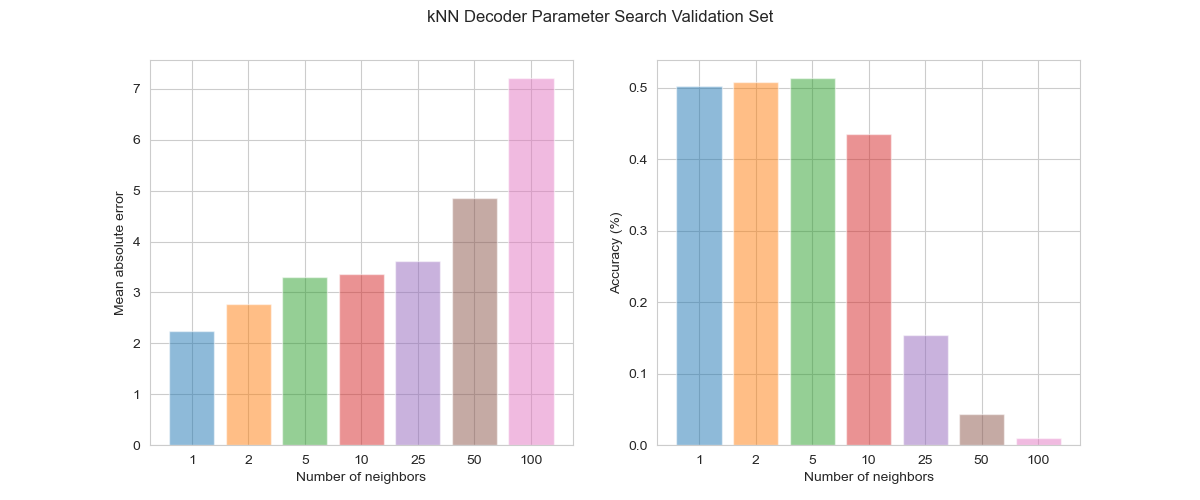
\includegraphics[width=1.0\textwidth]{cebra_latents_knn_decoder_grid_search.png}
    \caption{CEBRA KNN Neighbors Grid Search Validation Set}
    \label{fig:cebra_knn_frame_id_accuracy_mae}
\end{figure}

From the grid search we can see that the best number of neighbors for the KNN model was $1$ with the lowest MAE and highest accuracy. We then used the best number of neighbors to evaluate the KNN model on the test set and saw a $60\%$ accuracy and $.98$ MAE. If we compare that to \hyperref[fig:vae_frame_id_decoding_comparison]{Figure~\ref{fig:vae_frame_id_decoding_comparison}} we can see that the CEBRA \cite{schneider2023} latents are significantly better at decoding the frame ID compared to the VAE latents using KNN. The best performing KNN accuracy was $4\%$ and the lowest MAE was $16$ which means CEBRA \cite{schneider2023} latents are roughly $15$ times better at decoding the frame ID compared to the VAE latents. We also generated the first $10$ predicted frame IDs using the KNN model on the held out test set.

\begin{figure}[H]
    \centering
    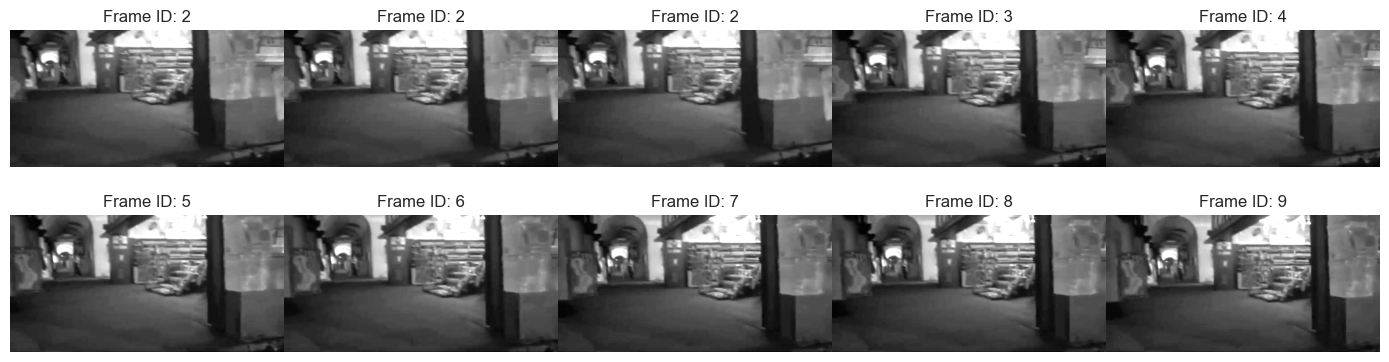
\includegraphics[width=1.0\textwidth]{cebra_knn_video.png}
    \caption{CEBRA KNN Decoded Frames}
    \label{fig:cebra_knn_frame_id_decoded_video}
\end{figure}

We can see that the CEBRA \cite{schneider2023} latents correctly predicted the frame ID for all frames except for the first and second frame. The first frame was predicted as frame ID $2$ and the second frame was predicted as frame ID $2$ as well. Comparing this to the VAE latents which predicted multiple frame IDs that were actually occurring much later in the video to be the first three frames in \hyperref[fig:vae_frame_id_decoded_video]{Figure~\ref{fig:vae_frame_id_decoded_video}}. 

\subsubsection{CEBRA Frame ID Decoding Logistic Regression}
\label{subsubsec:cebra_frame_id_decoding_logistic}
We also evaluated the CEBRA \cite{schneider2023} latents using logistic regression to decode the frame ID. We used $9$ training presentations and $1$ test presentation as mentioned before and plotted the train and test accuracy and MAE.

\begin{figure}[H]
    \centering
    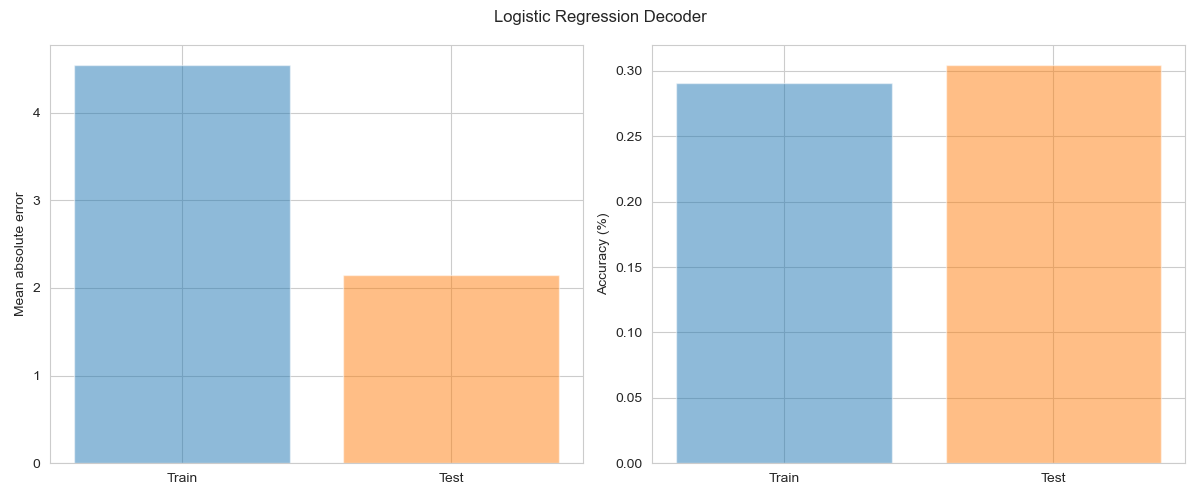
\includegraphics[width=.8\textwidth]{cebra_latents_lr_decoder.png}
    \caption{CEBRA Logistic Regression Frame ID Decoding}
    \label{fig:cebra_logistic_frame_id_accuracy_mae}
\end{figure}

Using a logistic regression model we see overall higher MAE and lower accuracy compared to KNN on the CEBRA \cite{schneider2023} latents with a $30\%$ accuracy and $2$ MAE on the test set. However, these results are still significantly better than the VAE latents which from \hyperref[fig:vae_frame_id_decoding_comparison]{Figure~\ref{fig:vae_frame_id_decoding_comparison}} had a best accuracy around $3.2\%$ and a best MAE of $18$. The CEBRA \cite{schneider2023} latents are roughly $10$ times better at decoding the frame ID compared to the VAE latents using logistic regression.

\subsubsection{CEBRA Neural Reconstruction}
\label{subsubsec:cebra_neural_reconstruction}
In order to validate the final step of understanding whether or not CEBRA \cite{schneider2023} latents are actually neural aligned we wanted to see how well the CEBRA \cite{schneider2023} latents are able to reconstruct the neural responses. We again split the $9$ training presentations into $7$ training and $2$ validation sets and plotted the $R^2$ score for the neural reconstruction on the validation and training sets. The decoder network was an MLP with LeakyReLU activations and the loss was the mse loss between the reconstructed neural responses and the true neural responses. After some exploration we found the best architecture to be $3$ layers in the decoder network. First, we used the full set of $772$ neuropixel responses as the target for the decoder network. Below are the results of the CEBRA \cite{schneider2023} latents neural reconstruction.

\begin{figure}[H]
    \centering
    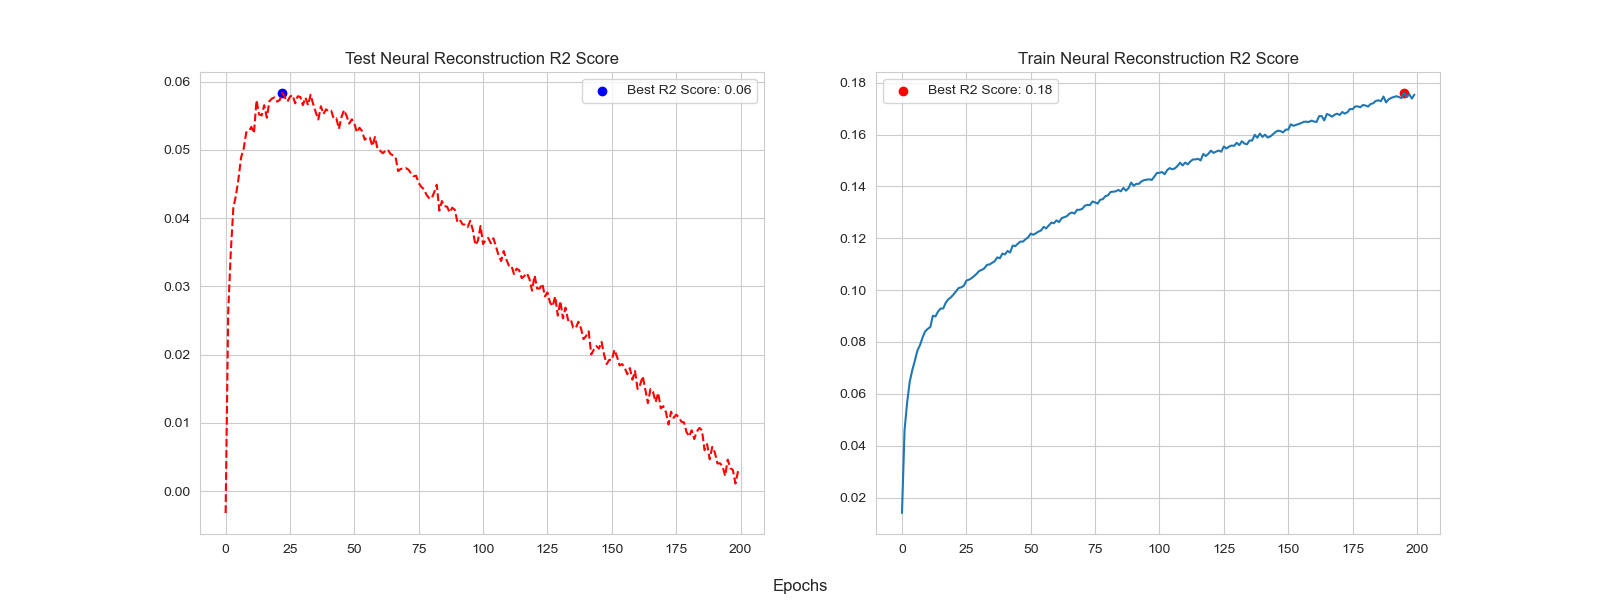
\includegraphics[width=1.0\textwidth]{cebra_x_r2_772_200_epochs_3_layer.png}
    \caption{CEBRA Latents Neural Reconstruction $R^2$ Score for Full Set of Neuropixels}
    \label{fig:cebra_latents_neural_reconstruction_772}
\end{figure}

The test set results above are measured on the $2$ presentation validation set. We can see that the CEBRA \cite{schneider2023} latents are unable to capture the variance in the neural responses with the best validation set $R^2$ score at $.06$. If you compare that to the VAE model without guidance on the latents which had a peak of $.32$ see \hyperref[fig:vae_no_guidance]{Figure~\ref{fig:vae_no_guidance}}. Even with guidance on the DINO \cite{dino} embeddings the VAE model was able to achieve a peak $R^2$ score of $.2$ see \hyperref[fig:vae_guidance_DINO_pca_full_neuropixels]{Figure~\ref{fig:vae_guidance_DINO_pca_full_neuropixels}}. We can also measure the CEBRA \cite{schneider2023} latent's ability to reconstruct the top $503$ neuropixels based on variance.

\begin{figure}[H]
    \centering
    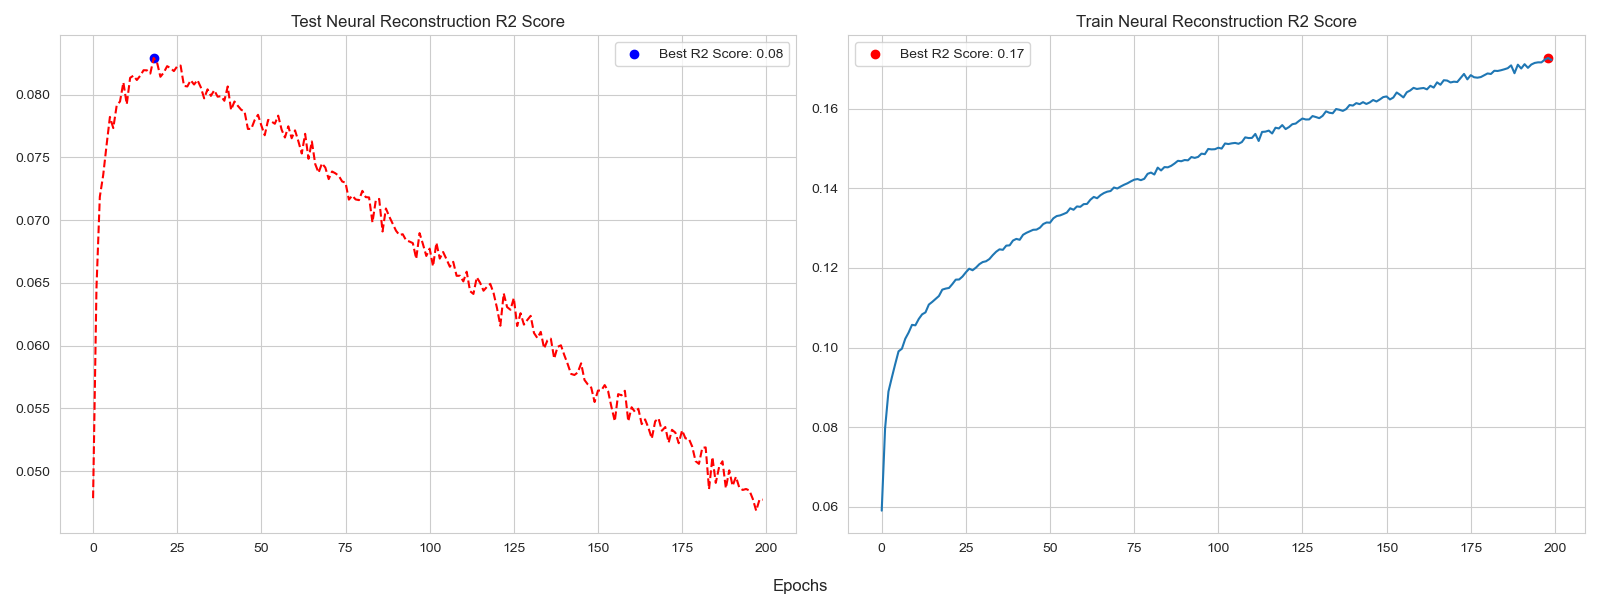
\includegraphics[width=1.0\textwidth]{cebra_x_r2_503_200_epochs_3_layer.png}
    \caption{CEBRA Latents Neural Reconstruction $R^2$ Score for Top $503$ Neuropixels}
    \label{fig:cebra_latents_neural_reconstruction_503}
\end{figure}

There is a slight improvement in the validation set $R^2$ score when using the top $503$ neuropixels compared to the full set of $772$ neuropixels most likely because the lower dimensionality of the neural responses. However, the best validation set $R^2$ score is still quite low at $.08$. If we compare that to \hyperref[fig:vae_no_guidance_top503]{Figure~\ref{fig:vae_no_guidance_top503}} we can see that the VAE model without guidances on the latents is able to achieve a much higher peak $R^2$ score of $.47$. Finally we also explore the CEBRA \cite{schneider2023} latents reconstruction of the top $393$ neuropixels based on variance.

\begin{figure}[H]
    \centering
    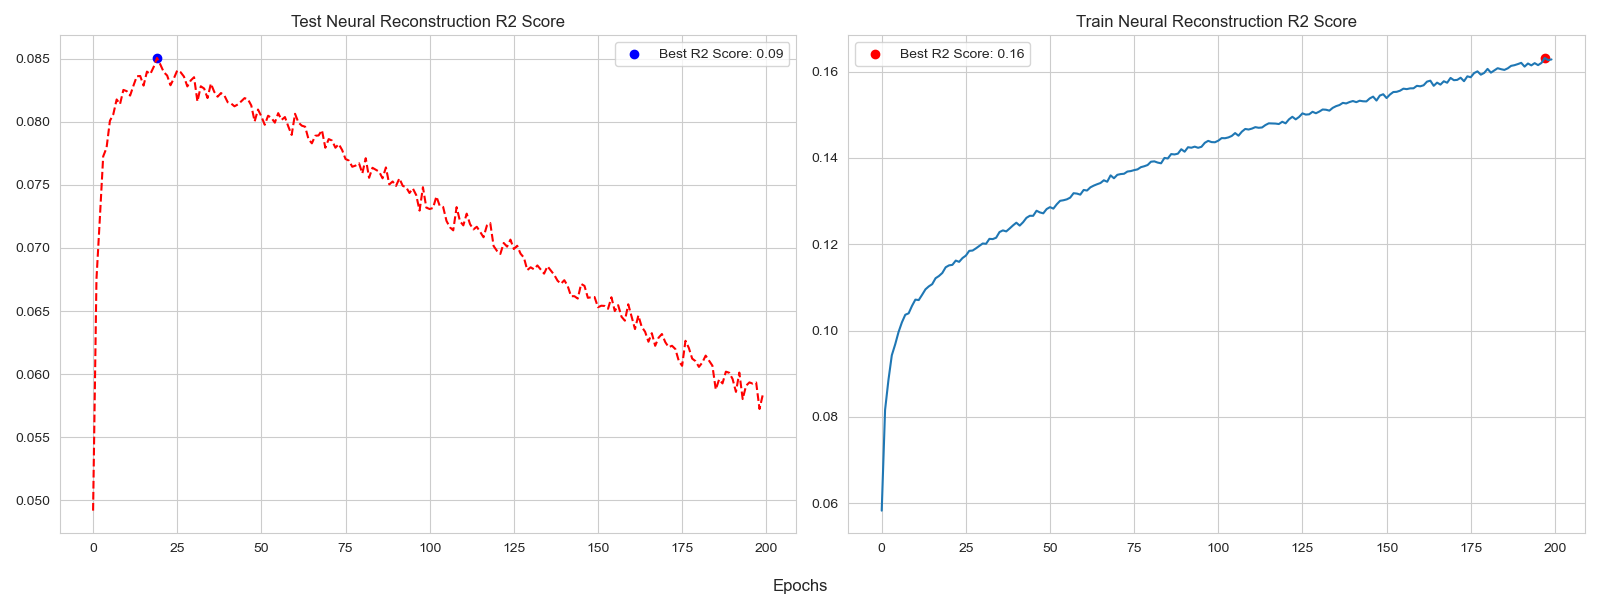
\includegraphics[width=1.0\textwidth]{cebra_x_r2_393_200_epochs_3_layer.png}
    \caption{CEBRA Latents Neural Reconstruction $R^2$ Score for Top $393$ Neuropixels}
    \label{fig:cebra_latents_neural_reconstruction_393}
\end{figure}

Following a similar trend the validation set $R^2$ score is slightly higher when using the top $393$ neuropixels compared to the top $503$ neuropixels. The best validation set $R^2$ score is $.09$ which is still quite low. If we compare that to \hyperref[fig:vae_no_guidance_top393]{Figure~\ref{fig:vae_no_guidance_top393}} we can see that the VAE model without guidance on the latents is able to achieve a much higher peak $R^2$ score of $.47$.

Using the left out test set we evaluated the ability for the CEBRA latents to decode different number of neuropixels starting with the full set of $772$ neuropixels, then top $503$ neuropixels, and finally the top $393$ neuropixels. We used the same decoder network architecture as before and plotted the $R^2$ score for the neural reconstruction on the test set.

\begin{figure}[H]
    \centering
    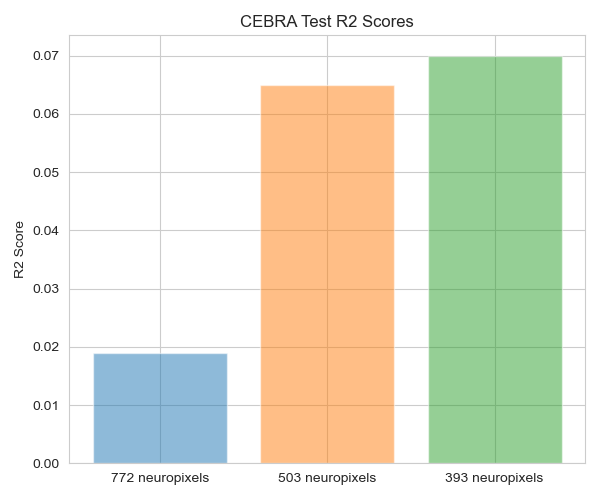
\includegraphics[width=0.6\textwidth]{cebra_test_r2_scores.png}
    \caption{CEBRA Latents Neural Reconstruction $R^2$ Score on Test Set}
    \label{fig:cebra_latents_neural_reconstruction_test_set}
\end{figure}

Similar to the validation set results the test set $R^2$ score is quite low for the CEBRA \cite{schneider2023} latents. The best test set $R^2$ score was $.07$ when decoding the top $393$ top variance neuropixels. We were only able to see a $.019$ $R^2$ score when decoding the full set of $772$ neuropixels and a $.065$ $R^2$ score when decoding the top $503$ neuropixels.

\section{Discussion}
\label{sec:discussion}
The key findings of our study can be broken down into the complexity and significance of learning frame IDs from neural responses and whether or not CEBRA \cite{schneider2023} latents are neurally aligned. We can conclude that learning the frame ID classification accurately is highly significant but is most likely not neurally aligned. If we look at the results of mapping from PCA components of neural responses to frame ID in \hyperref[subsec:pca_decoding]{\ref{subsec:pca_decoding}} and mapping from raw neural responses to frame ID in \hyperref[subsec:neuropixel_decoding]{\ref{subsec:neuropixel_decoding}} we can see that a linear mapping is able to predict roughly what the correct frame should be based on the $R^2$ scores but the accuracy is low and it is unable to fully discern the exact frame corresponding to a neural response. The VAE models also show similar results while we are able to have a decent neural reconstruction the frame ID MAE and accuracy are only marginally better than PCA or the raw neural response after using DINO embeddings as guidance on the latents shown in \hyperref[subsubsec:vae_guidance_DINO]{\ref{subsubsec:vae_guidance_DINO}}. The CEBRA \cite{schneider2023} model on the other hand is able to achieve significantly higher accuracy using both KNN and logistic regression to decode the frame ID demonstrated in \hyperref[subsubsec:cebra_frame_id_decoding_knn]{\ref{subsubsec:cebra_frame_id_decoding_knn}} and \hyperref[subsubsec:cebra_frame_id_decoding_logistic]{\ref{subsubsec:cebra_frame_id_decoding_logistic}}. However, when attempting to decode neural responses we can see that the CEBRA \cite{schneider2023} latents do not capture the variance in the neural responses nearly as well as the VAE models shown in \hyperref[subsubsec:cebra_neural_reconstruction]{\ref{subsubsec:cebra_neural_reconstruction}}. A biological explanation could be because these neural response originated from mouse V1 visual cortex which from the CEBRA \cite{schneider2023} paper showed the best frame ID decoding results. However, V1 being a low-level visual cortex would not actually encode for abstract representations of the stimulus which would be required to discern frames that are very similar. This leads us to believe that in reality the CEBRA \cite{schneider2023} latents are not neurally aligned and are more likely artificially embedded in a manner to maximize the separation. This result challenges the CEBRA \cite{schneider2023} papers findings of a high reconstruction performance on synthetic neural responses. While we did not directly benchmark CEBRA \cite{schneider2023} against pi-VAE which was the comparison made in the CEBRA \cite{schneider2023} literature we can see that for the baseline VAE model CEBRA \cite{schneider2023} latent decoding has a significantly lower reconstruction. This may also highlight that just using synthetic neural data isn't enough to properly benchmark a model's reconstruction performance. To highlight some limitations of our own study, the VAE model and decoder model architectures were not optimized and we could have potentially achieved better results with more tuning on the number of layers, layer sizes, and even leveraging more complex networks such as a recurrent VAE which might perform better because each frame and neural response is sequential. Our VAE reconstruction $R^2$ is notably lower than the cumulative explained variance using PCA shown in the explained variance curve so there definitely is more room to improve the VAE results with model tuning. In addition, the dataset had only $10$ presentations of $900$ frames which could explain why the VAE models with frame ID guidance performed poorly since each class or frame would only have at most $10$ samples. 

\section{Conclusion}
\label{sec:conclusion}
The main findings are that a VAE model even with supervision on the latents is not able to decode the frame ID as well as the CEBRA \cite{schneider2023} model. This most likely is due to the information that is encoded into low-level visual cortex like V1 is not rich enough to capture distinctions between very similar frames. From viewing the video many adjacent frames contain minute differences and would most likely only be captured in the response from a high level visual cortex. In addition, we found that CEBRA \cite{schneider2023} latents are not neurally aligned. While their performance on frame ID decoding is significantly better than PCA and VAE the latents had poor reconstruction when decoding to the original neural response. As a follow up it would interesting to explore our original VAE model implementation but on a higher level visual cortex in mice. We could also do the same exploration but for a different modality such as calcium imaging. Finally, we could explore CEBRA \cite{schneider2023} model's neural reconstruction on a different task instead of passive viewing potentially a behavioral task with motor cortex neural responses. 

\newpage
\begin{thebibliography}{9}
    % Schneider, S., Lee, J.H. & Mathis, M.W. Learnable latent embeddings for joint behavioural and neural analysis. Nature 617, 360–368 (2023). https://doi.org/10.1038/s41586-023-06031-6
    \bibitem{schneider2023}
    Schneider, S., Lee, J.H. \& Mathis, M.W. \textit{Learnable latent embeddings for joint behavioural and neural analysis}. Nature 617, 360–368 2023. \url{https://doi.org/10.1038/s41586-023-06031-6}

    % Primary publication: Siegle, J. H., Jia, X., Durand, S., et al. (2021). Survey of spiking in the mouse visual system reveals functional hierarchy. Nature, 592(7612), 86-92. https://doi.org/10.1038/s41586-020-03171-x | Dataset: Allen Institute MindScope Program (2019). Allen Brain Observatory -- Neuropixels Visual Coding [Dataset]. Available from brain-map.org/explore/circuits
    \bibitem{siegle2021}
    Siegle, J. H., Jia, X., Durand, S., et al. \textit{Survey of spiking in the mouse visual system reveals functional hierarchy}. Nature, 592(7612), 86-92, 2021. \url{https://doi.org/10.1038/s41586-020-03171-x}
    
    \bibitem{cebra_demo}
    CEBRA Demo. \textit{Decoding movie features from (V1) visual cortex}. Accessed: November, 2024. Available at: \url{https://cebra.ai/docs/demo_notebooks/Demo_Allen.html#Decoding-movie-features-from-(V1)-visual-cortex}

    % @article{DBLP:journals/corr/abs-2104-14294,
    % author       = {Mathilde Caron and
    %                 Hugo Touvron and
    %                 Ishan Misra and
    %                 Herv{\'{e}} J{\'{e}}gou and
    %                 Julien Mairal and
    %                 Piotr Bojanowski and
    %                 Armand Joulin},
    % title        = {Emerging Properties in Self-Supervised Vision Transformers},
    % journal      = {CoRR},
    % volume       = {abs/2104.14294},
    % year         = {2021},
    % url          = {https://arxiv.org/abs/2104.14294},
    % eprinttype    = {arXiv},
    % eprint       = {2104.14294},
    % timestamp    = {Tue, 04 May 2021 15:12:43 +0200},
    % biburl       = {https://dblp.org/rec/journals/corr/abs-2104-14294.bib},
    % bibsource    = {dblp computer science bibliography, https://dblp.org}
    % }
    \bibitem{dino}
    Caron, M., Touvron, H., Misra, I., Jégou, H., Mairal, J., Bojanowski, P., \& Joulin, A. \textit{Emerging Properties in Self-Supervised Vision Transformers}. CoRR, abs/2104.14294, 2021. \url{https://arxiv.org/abs/2104.14294}

\end{thebibliography}

\end{document}
